\documentclass[10pt]{beamer}

%STANDARD PREAMBLE
%https://tex.stackexchange.com/questions/68821/is-it-possible-to-create-a-latex-preamble-header
\usepackage{/Users/mwojno01/Research/Learning/latex_preamble/beamer_preamble}



%
%% ALLOW FOR ITEMIZE ENVIRONMENTS WITH NO PRECEDING
% SPACING, IF DESIRED
% Reference: https://tex.stackexchange.com/questions/86054/how-to-remove-the-whitespace-before-itemize-enumerate
%\usepackage{enumitem}% http://ctan.org/pkg/enumitem 
\usepackage{paralist}

\title{Unit tests in python}

\begin{document}

\maketitle

\begin{frame}{Some good practices}

\begin{itemize}
\item Run tests before committing changes to source code. 
\item Should be \alert{fast} (5-10 seconds to run \textit{all} tests).
\item Each test function name should have a postfix describing what we're testing:
	\begin{center}\url{test__function_name__what_property_we_are_testing}	
	\end{center}
\item One assertion per test.
\end{itemize} 
\end{frame}

\section{The \texttt{hypothesis} package}

\begin{frame}
\begin{center}
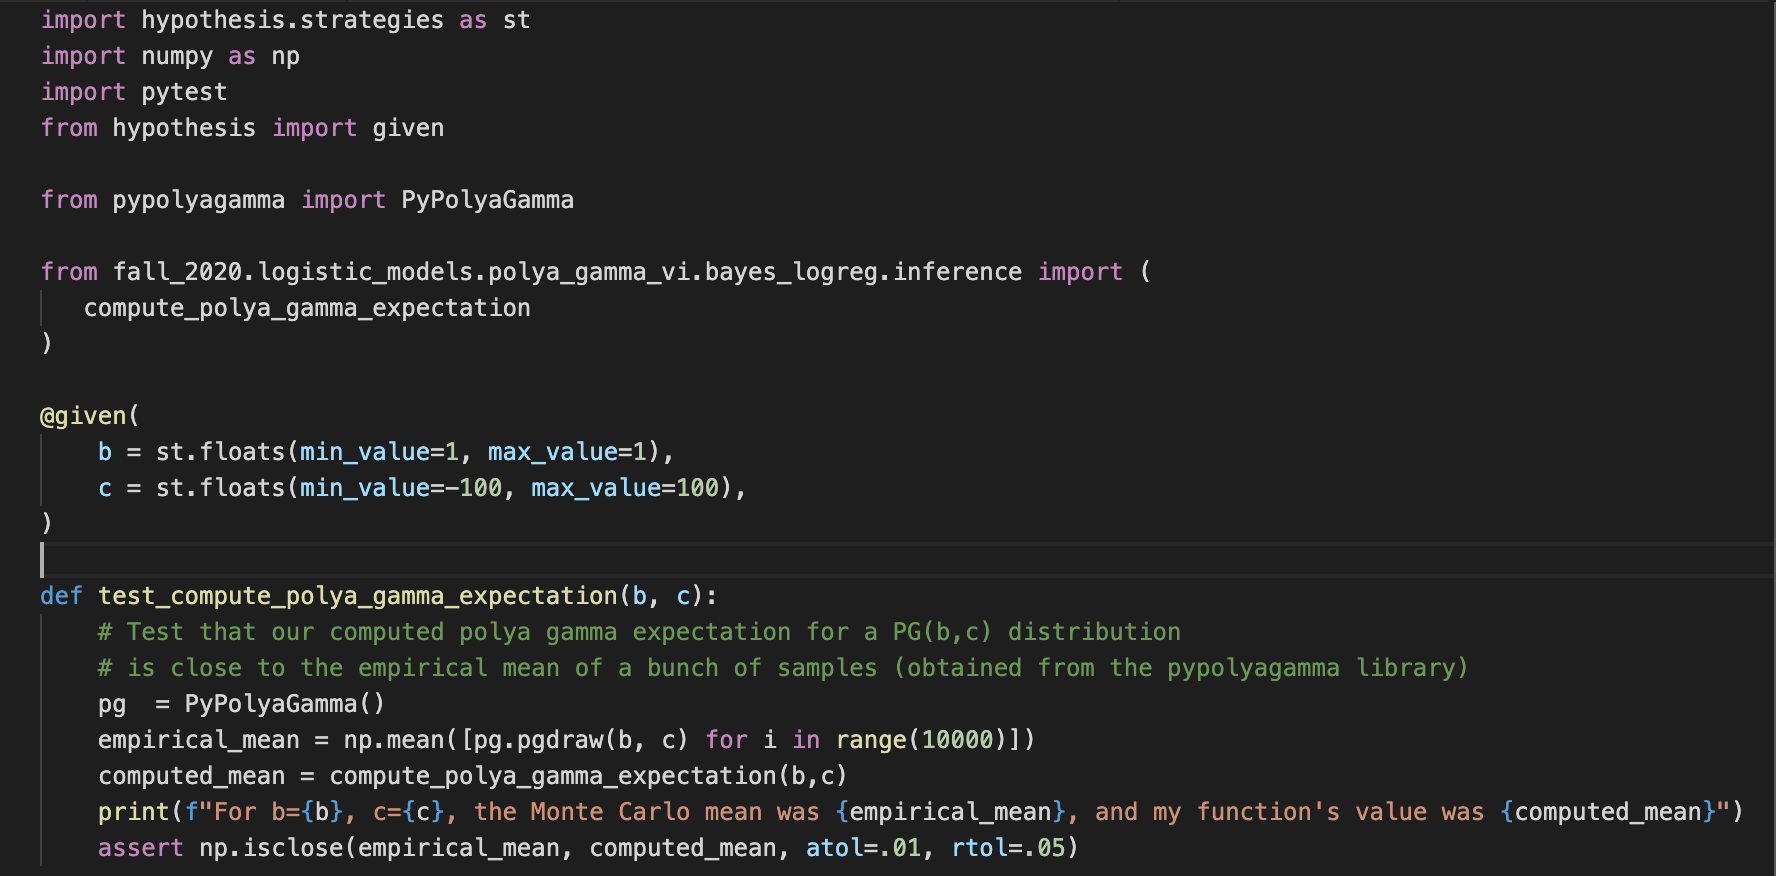
\includegraphics[width=\textwidth]{images/pypolyagamma_test}	
\end{center}
	
\end{frame}

\begin{frame}
\begin{center}
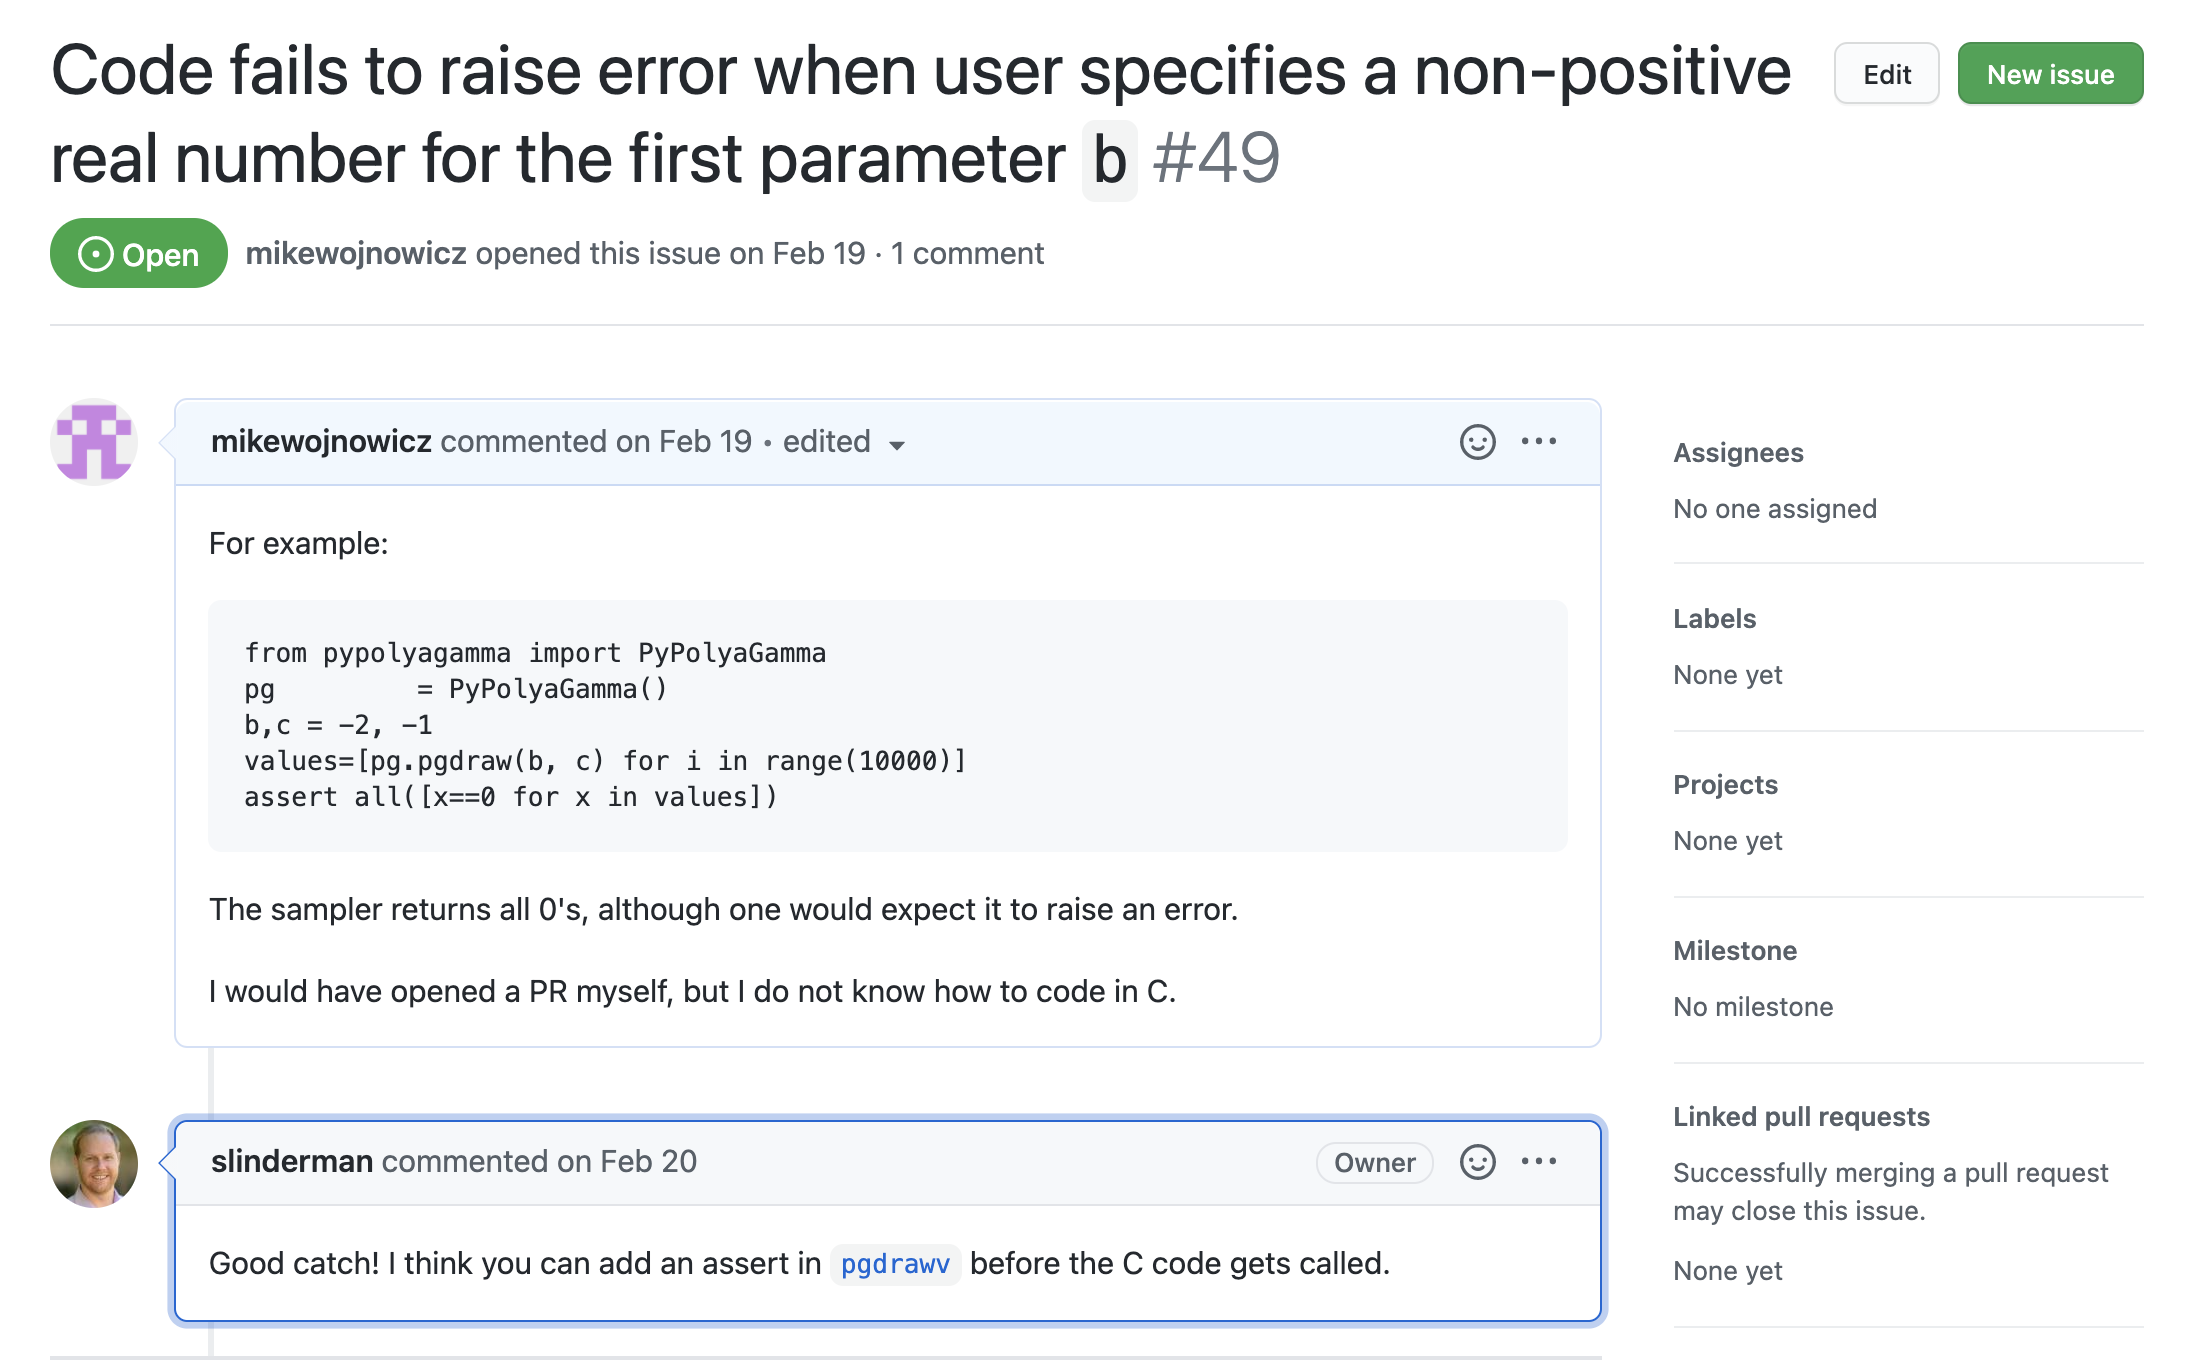
\includegraphics[width=\textwidth]{images/pypolyagamma_issue}	
\end{center}
	
\end{frame}




\end{document}